\section{A Hybrid Model of Prostate Cancer Progression }\label{sec.model}

In this section, we propose a hybrid automata based model in order to reproduce the clinical observations \cite{bruchovsky06, bruchovsky07} of prostate cancer cell dynamics in response to the IAS therapy. It is known that the proliferation and survival of prostate cancer cells depend on the levels of androgens, specifically testosterone and 5$\alpha$-dihydrotestosterone (DHT).
Here we consider two distinct subpopulations of prostate cancer cells: hormone sensitive cells (HSCs) and castration resistant cells (CRCs). Androgen deprivation can lead to remarkable decreases of the proliferation and survival rates of HSCs, but also up-regulates the conversion from HSCs to CRCs, which will keep proliferating under low androgen level. %Figure \ref{progression} illustrates this cancer progression process and the corresponding hybrid automata model is shown in Figure \ref{pmodel}. 
The corresponding hybrid automata model is shown in Figure \ref{pmodel}. 


%\begin{figure}[htb]
%\centering
%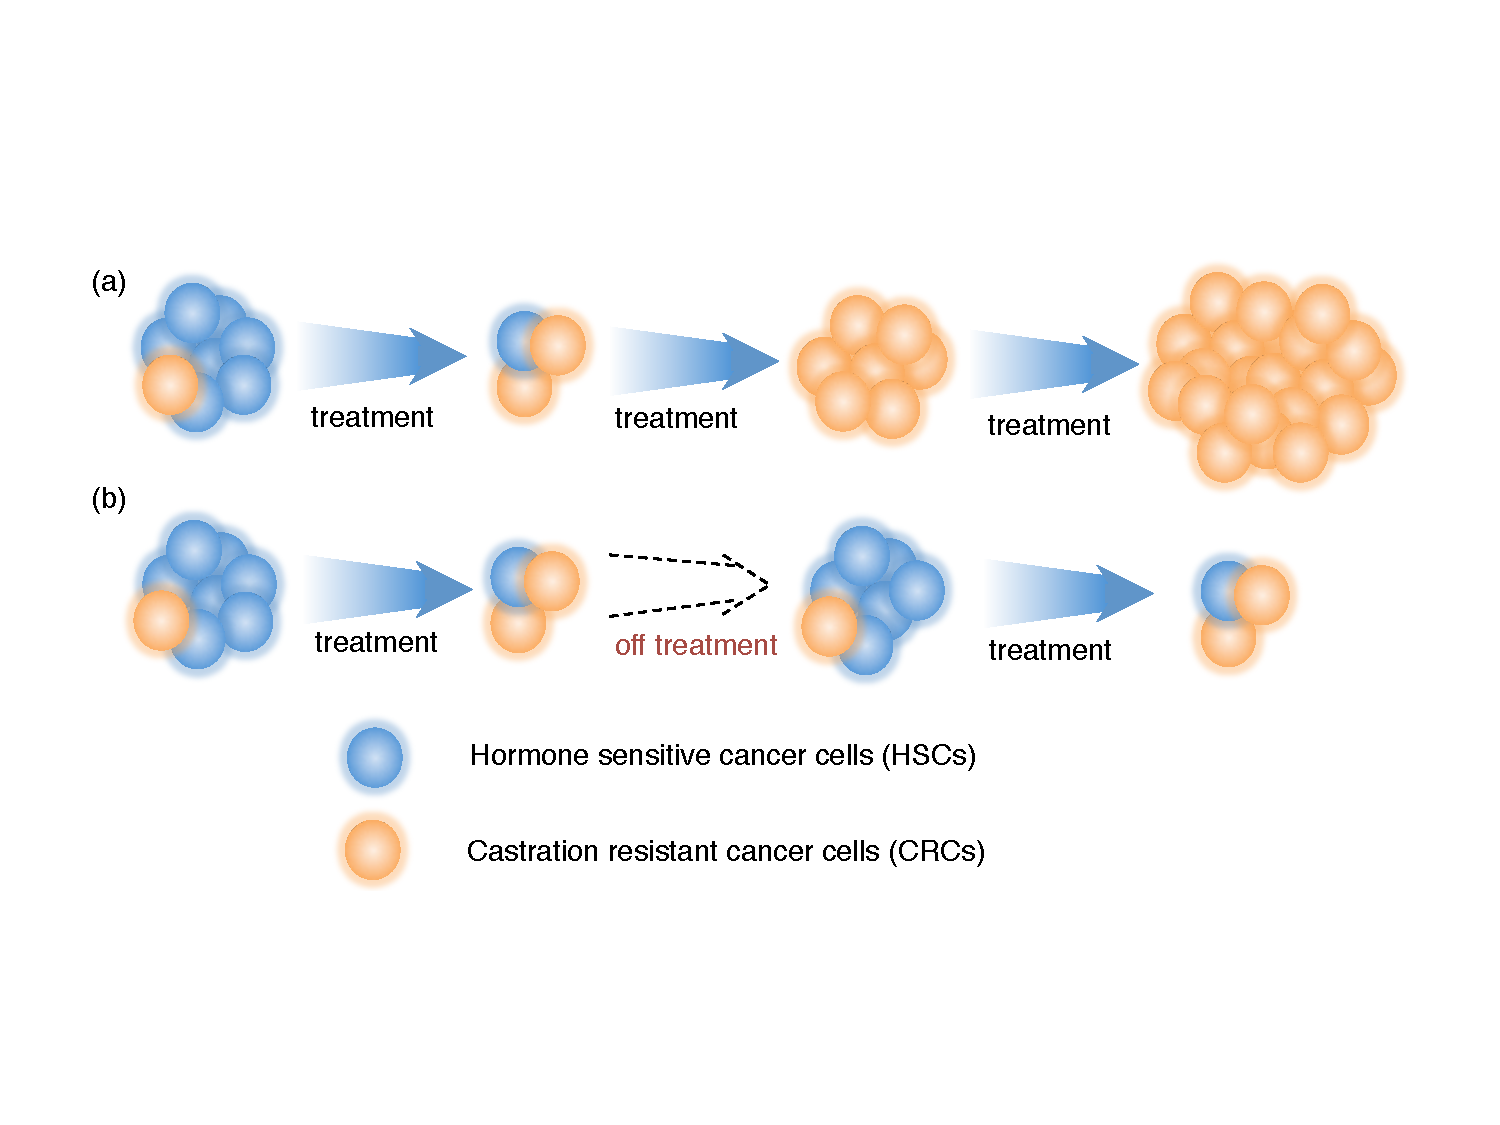
\includegraphics[scale=0.38]{fig-progression}
%\caption{Prostate cancer progression in response to (a) CAS and (b) IAS treatments.}
%\label{progression}
% %\vspace{-0.1cm}
%\end{figure}

\begin{figure}[htb]
\centering
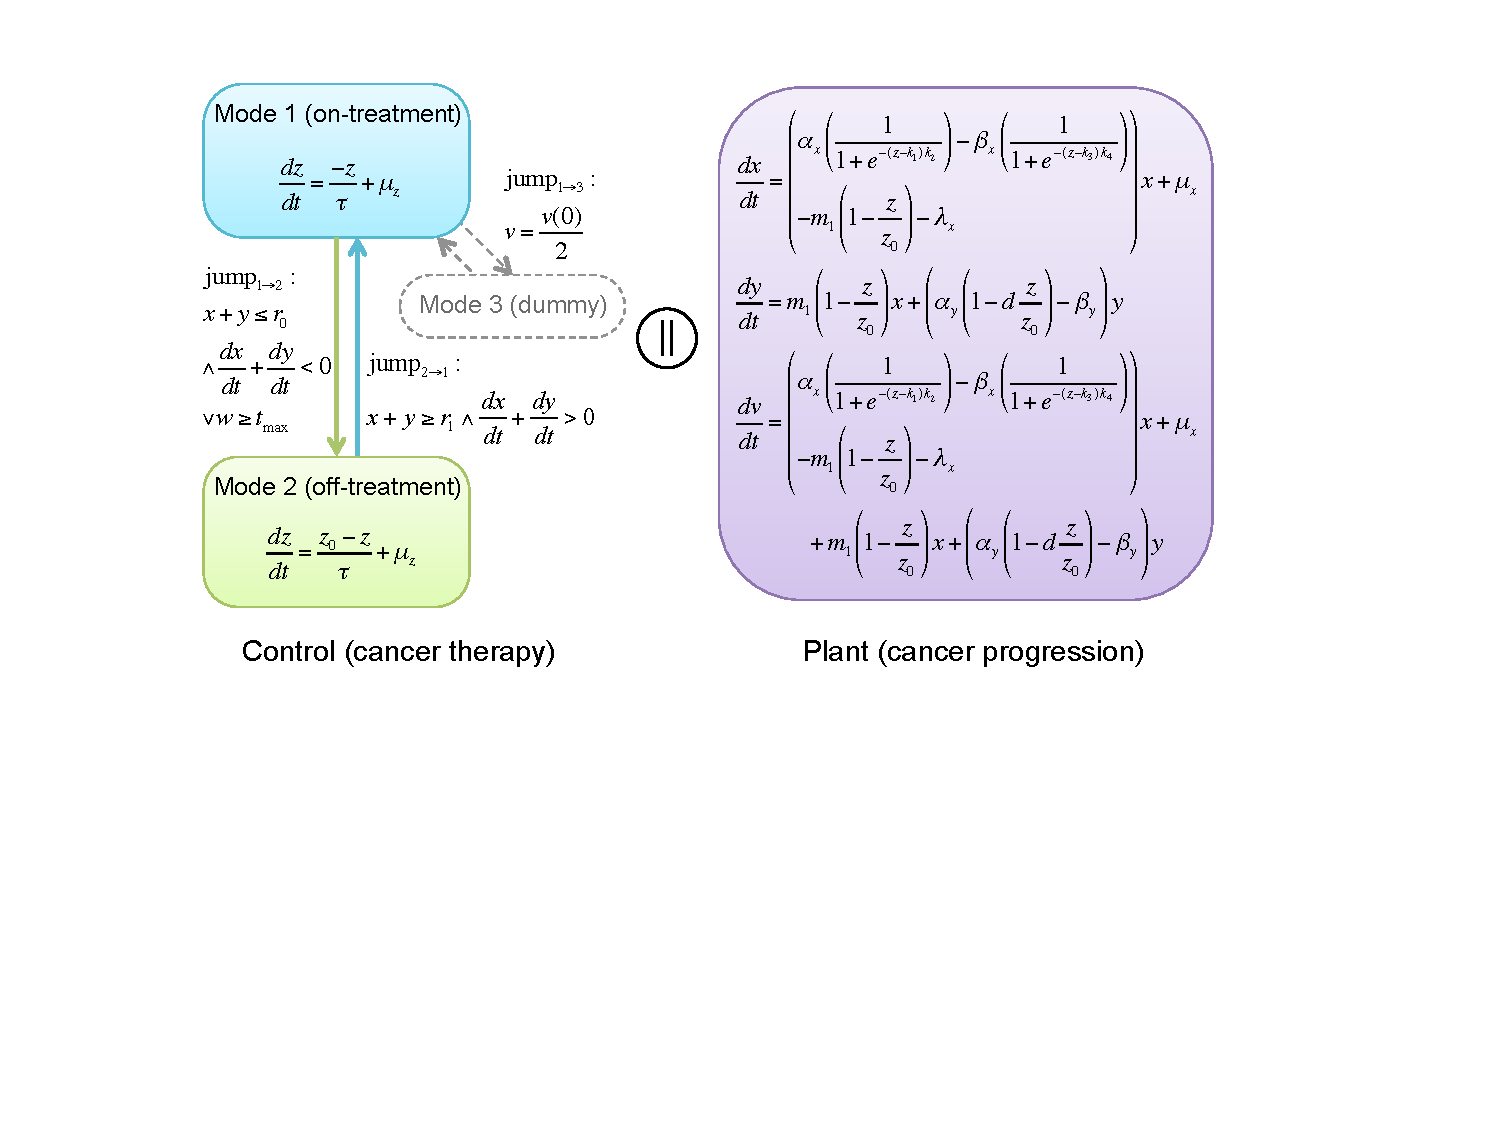
\includegraphics[scale=0.55]{fig-prostate3}
\caption{A hybrid automaton model for prostate cancer hormone therapy.}
\label{pmodel}
 \vspace{-0.3cm}
\end{figure}


% Reviewer#1
% Section 2 describes a 2 modes hybrid automaton, but later Section 4.2 presents a further modified automaton with 3 modes. It might be clearer to have the final version in Section 2 and Figure 2.

% Reviewer#2
% Figure 2: The dynamics for mode 1 and 2 appear to differ only in dz/dt and also differ depending on the jump direction. This figure could be greatly consolidated and the differences more clearly highlighted.

Our model is based on previous models developed by \cite{jackson04a,jackson04b,ideta08}. It takes into account the population of HSCs, the population of CRCs, as well as the serum androgen concentration, represented as $x(t)$, $y(t)$, and $z(t)$, respectively. In addition, it also includes the serum prostate-specific antigen (PSA) level $v(t)$, which is a commonly used biomarker for assessing the total population of prostate cancer cells. The model has two modes: \textit{on-treatment} mode and \textit{off-treatment} mode. Following \cite{ideta08}, in the off-treatment mode (mode $2$), the androgen concentration is maintained at the normal level $z_0$ by homeostasis. In the on-treatment (mode $1$), the androgen is cleared at a rate $\frac{1}{\tau}$. Further, we also introduce a basal androgen production rate $\mu_z$, in order to reproduce the measured basal testosterone levels in response to androgen suppression \cite{bruchovsky06, bruchovsky07}. 

The net growth rate of $x(t)$ equals to $(prolif_{x}-apop_{x}-conv_{x})\cdot x(t)$, where $prolif_x$, $apop_x$ and $conv_x$ denote the proliferation, apoptosis and conversion rates, respectively. In previous studies such as \cite{jackson04a,jackson04b,ideta08}, the $prolif_x$ and $apop_x$ were modeled using Michaelis-Menten-like (MML) functions, in the form of $V_{max}+(1-V_{max})\frac{z(t)}{z(t)+K_{m}}$, where $V_{max}$ and $K_m$ are kinetic parameters. This approach will result in androgen response curves as shown in Figure \ref{response}(a). In particular, when one decreases the androgen level starting from the normal level, $prolif_x$ (or $apop_x$) begins to decrease (or increase) first slowly and then fast until a sufficiently low level of androgen is reached. However, this is inconsistent with the clinical observations presented in \cite{bruchovsky06, bruchovsky07}. The data show that for most of the patients, androgen suppression around normal level will induce an immediate decrease of the PSA level, which implies an fast decrease (or increase) of $prolif_x$ (or $apop_x$). Therefore, instead of the MML functions, we adopt sigmoid functions, in the form of  $\frac{1}{1+exp(-(z(t)-k_1)\cdot k_2)}$, to model $prolif_x$ and $apop_x$. The corresponding androgen response curves are shown in Figure \ref{response}(b). Following \cite{ideta08}, we model the conversion rate, proliferation rate and the apoptosis rate of $y(t)$ as $m_1(1-\frac{z(t)}{z_0})$, $\alpha_y(1-d\frac{z(t)}{z_0})$ and $\beta_y$, respectively. The PSA level $v$ (ng ml$^{-1}$) is defined as $v(t)=c_1\cdot x(t)+c_2\cdot y(t)$. 

\begin{figure}[htb]
\centering
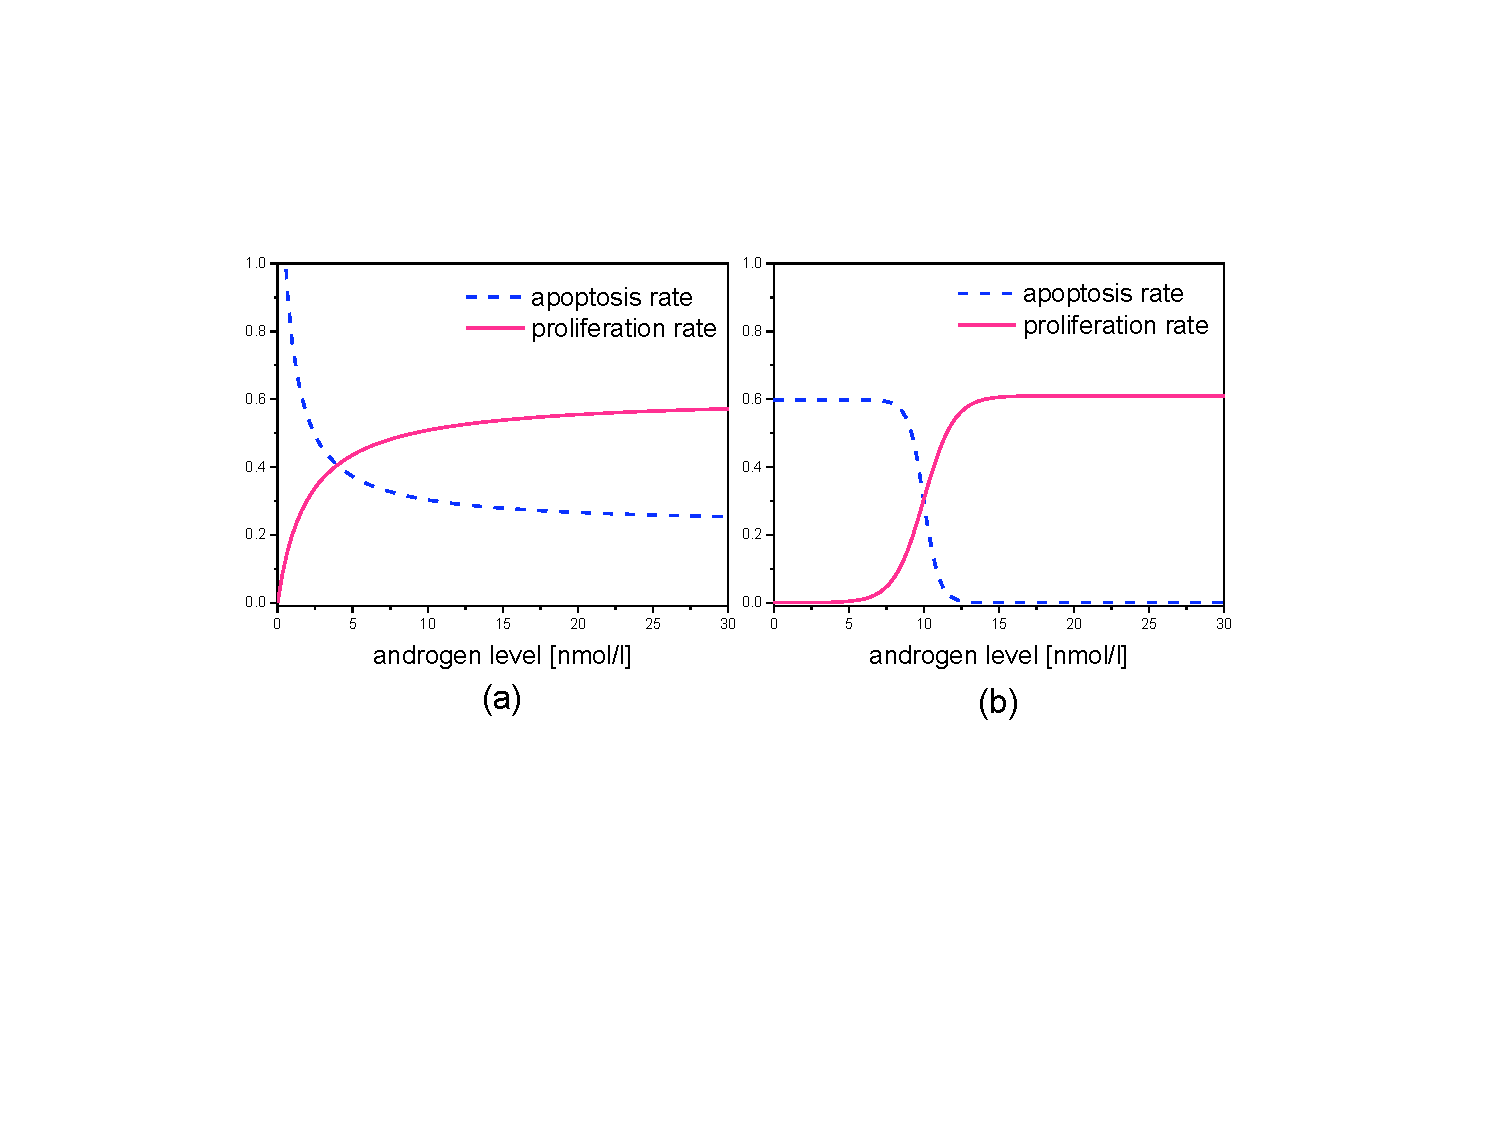
\includegraphics[scale=0.45]{fig-response}
\caption{Androgen response curves of (a) Ideta's model and (b) our model.}
\label{response}
% \vspace{-0.3cm}
\end{figure}



The transitions between two modes depends on the values of $v$, ${dv}/{dt}$ and an auxiliary variable $w$, which measures the time taken in a mode. Specifically, for each patient we starts with mode $1$ to apply the treatment. When the PSA level drops to certain threshold $r_0$ or $w$ hits time out threshold $t_{max}$, the treatment will be suspended. When the PSA level is back to threshold $r_1$, the treatment will be resumed. Note that $w$ is associated with a dummy differential equation $\frac{dw}{dt}=1$ (not shown in Figure \ref{pmodel}). Its value will be reset to $0$ when the jump takes place.  

We obtained the parameter values by fitting to patient PSA data reported in \cite{bruchovsky06, bruchovsky07}. Note that the patient-to-patient variability in terms of parameter values is significant. For example, Figure \ref{data} shows that the proliferation rate of Patient\#22 is much lower than the Patient\#1. The descriptions and a set of typical values (i.e. estimated from Patient\#1 data) of model parameters are listed in Table \ref{prostate}.

\begin{figure}[htb]
\centering
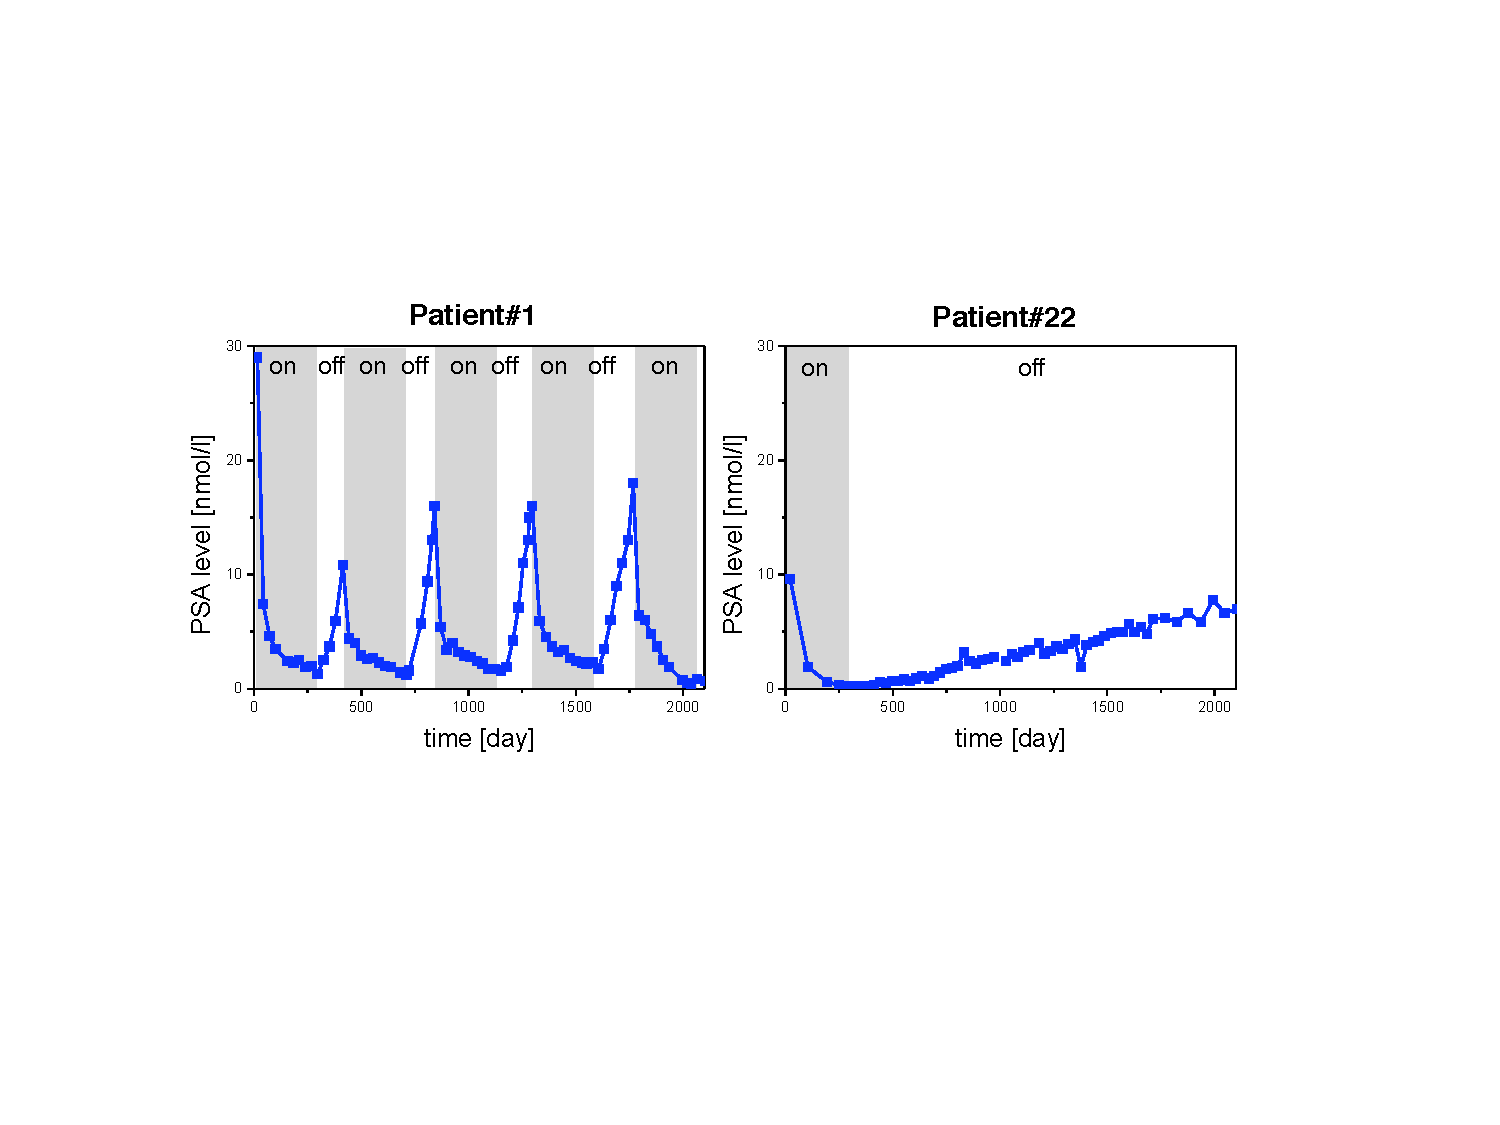
\includegraphics[scale=0.45]{fig-data}
\caption{The clinical data for PSA time serials.}
\label{data}
 \vspace{-0.3cm}
\end{figure}




\begin{table}[ht]
\caption{Prostate cancer model parameter values\label{prostate}}
\centering
\small
\begin{tabular}{|c|c|c|}
\hline
Parameter  & Value & Remark  \\\hline
$\alpha_x$ & 0.0204 d$^{-1}$ & HSC proliferation \\
$\alpha_y$ & 0.0242 d$^{-1}$ & CRC proliferation  \\
$\beta_x$  & 0.0201 d$^{-1}$ & HSC apoptosis  \\
$\beta_y$  & 0.0168 d$^{-1}$ & CRC apoptosis \\
$k_1$     & 10.0 nM & HSC proliferation  \\
$k_2$     & 1.0 & HSC proliferation  \\
$k_3$     & 10.0 nM & HSC apoptosis  \\
$k_4$     &  2 & HSC apoptosis   \\
$m_1$     & 0.00005 d$^{-1}$ & HSC to CRC conversion  \\
$z_0$     & 12.0 nM & normal androgen level  \\
$\tau$     & 12.5 d & androgen degradation  \\
$\lambda_x$     & 0.01 d$^{-1}$ & HSC basal degradation \\
$\mu_x$     & 0.05 d$^{-1}$ & HSC basal production\\
$\mu_z$     & 0.02 d$^{-1}$ & Androgen basal production \\
\hline
\end{tabular}
% \vspace{-0.5cm}
\end{table}
